\chapter{Umfrage Daten}
%\begin{center}
%	\begin{table}[h]
%		\begin{tabularx}{4cm}{|l|l|p{4.5 cm}|ll}
%			\cline{1-3}
%			\textbf{Technolgie} & \textbf{Vorteil}                         & \textbf{Nachteil}                                                &  &  \\ \cline{1-3}
%			Angular             & Schlanker Kerncode mit hoher Modularität & nicht geeignet für dynamiche Web-App  &  &  \\ \cline{1-3}
%			React               & Einfach zu erlernen, aktive Community    & Weniger leistungsstark         &  &  \\ \cline{1-3}
%			Vue.js              & Einfache Satzlehre, schnelle Startzeit   & Kleinere Community             &  &  \\ \cline{1-3}
%		\end{tabularx}
%	\end{table}
%\end{center}+
\section{Frage 1}
\begin{wrapfigure}[2]{r}{0.5\textwidth}
	\centering
	\fbox{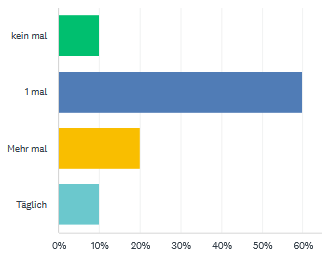
\includegraphics[width=0.4\textwidth]{images/frage-01}}
\end{wrapfigure}
\textbf{Frage:} Wie oft hast du DHBW Star in den letzten 7 tagen benutzt?\\
\textbf{Ergebnisse:}\\
\begin{tabular}{|l|c|}\hline
	\textbf{Antwortoptionen} & \textbf{Beantwortungen} \\\hline
	kein mal & 1 \\\hline
	1 mal	 & 6 \\\hline
	Mehr mal & 2 \\\hline
	Täglich  & 1 \\\hline
	GESAMT	 & 10 \\\hline			
\end{tabular}
%\begin{figure}[htbp]
%	\fbox{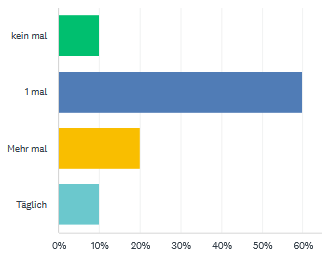
\includegraphics[width=0.45\textwidth]{images/frage-01}}
%\end{figure}



\section{Frage 2}
\begin{wrapfigure}[2]{r}{0.5\textwidth}
	\centering
	\fbox{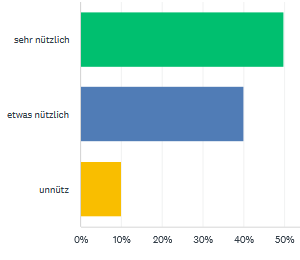
\includegraphics[width=0.40\textwidth]{images/frage-02}}
\end{wrapfigure}
\textbf{Frage:} Auf welchem gerät hast du DHBW Star benutzt?\\
\textbf{Ergebnisse:}\\
\\
\begin{tabular}{|l|c|}\hline
	\textbf{Antwortoptionen} & \textbf{Beantwortungen} \\\hline
	PC 			& 8 \\\hline
	Tablet		& 0 \\\hline
	Mobile 		& 4 \\\hline
	GESAMT		& 10 \\\hline			
\end{tabular}

\section{Frage 3}
\begin{wrapfigure}[2]{r}{0.5\textwidth}
	\centering
	\fbox{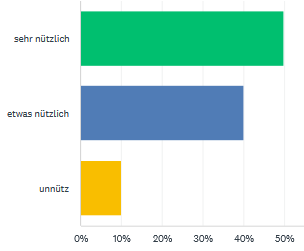
\includegraphics[width=0.40\textwidth]{images/frage-03}}
\end{wrapfigure}

\textbf{Frage:} Wie nützlich findest du die Startseite?\\
\textbf{Ergebnisse:}\\
\\
\begin{tabular}{|l|c|}\hline
	\textbf{Antwortoptionen} & \textbf{Beantwortungen} \\\hline
	sehr nützlich  	& 5 \\\hline
	etwas nützlich	& 4 \\\hline
	unnütz 			& 1 \\\hline
	GESAMT			& 10 \\\hline			
\end{tabular}

\section{Frage 4}
\textbf{Frage:} Wie gefällt dir die Darstellung des 'Scheduler' im verglich zum Rapla?
\begin{wrapfigure}[2]{r}{0.5\textwidth}
	\centering
	\fbox{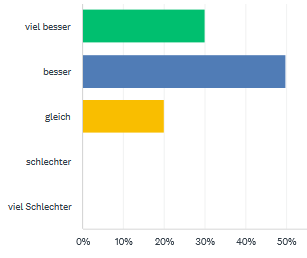
\includegraphics[width=0.40\textwidth]{images/frage-04}}
\end{wrapfigure}
\textbf{Ergebnisse:}\\
\\
\begin{tabular}{|l|c|}\hline
	\textbf{Antwortoptionen} & \textbf{Beantwortungen} \\\hline
	viel besser  	& 3 \\\hline
	besser			& 5 \\\hline
	gleich 			& 2 \\\hline
	schlechter 		& 0 \\\hline
	viel Schlechter	& 0 \\\hline
	GESAMT			& 10 \\\hline			
\end{tabular}

\section{Frage 5}
\textbf{Frage:} Was gefällt oder fehlt dir beim Scheduler?\\
\begin{tabular}{|l|}\hline
	\textbf{Antworten} \\\hline
	Simples Design nicht zu überladen / Tages Funktion cool  \\\hline
	ein paar Bugs verbessern, schon visualisiert week und day ansicht \\\hline
	Direkter Link zu EvaSys der Vorlesung :D \\\hline
	Die Räume fehlen zumindest auf Mobile und eine Auswahl der Wahlmodule wäre\\
	praktisch, da man wenn alle angezeigt werden die Freitagsmodule kaum lesen kann 
	\\\hline
	Fehlt: Dozenten, Raum, Individualisierung (nicht jeder hat jede Vorlesung) \\\hline
	Filter für kurse \\\hline			
\end{tabular}

\section{Frage 6}
\textbf{Frage:} Wie gefällt dir die Darstellung des Food im verglich zum sw-ka.de?
\begin{wrapfigure}[1]{r}{0.5\textwidth}
	\centering
	\fbox{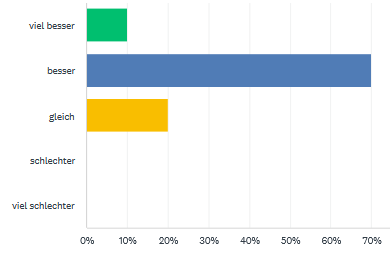
\includegraphics[width=0.40\textwidth]{images/frage-06}}
\end{wrapfigure}
\textbf{Ergebnisse:}\\
\\
\begin{tabular}{|l|c|}\hline
	\textbf{Antwortoptionen} & \textbf{Beantwortungen} \\\hline
	viel besser  	& 1 \\\hline
	besser			& 7 \\\hline
	gleich 			& 2 \\\hline
	schlechter 		& 0 \\\hline
	viel Schlechter	& 0 \\\hline
	GESAMT			& 10 \\\hline			
\end{tabular}

\section{Frage 7}
\textbf{Frage:} Was gefällt oder fehlt dir beim Food?\\
\begin{tabular}{|l|}\hline
	\textbf{Antworten} \\\hline
	Simpel nicht zu überladen  \\\hline
	emojis, benutzerfreundlich , schön gesammelt in einem ort \\\hline
	Ich sehe direkt was es in der Mensa hier an der DH gibt \\\hline
	die simple Darstellung ist toll, was man noch hinzufügen könnte wäre ein\\
	heute knopf oder so, da aktuell ja nur die Daten drin stehen 
	\\\hline
	Fehlt: "Heute"-Button, Tage (Montag/Dienstag/...)\\
	Gefällt: Man muss sich nicht erst durch einen Haufen Links klicken bis man zum Essen kommt. \\\hline
	Wochentagbezeichnung, nachhaltigkeitsbewertungen, allergien und so \\\hline			
\end{tabular}

\section{Frage 8}
\textbf{Frage:} Wie nützlich findest du die Link-Sammlung?
\begin{wrapfigure}[2]{r}{0.5\textwidth}
	\centering
	\fbox{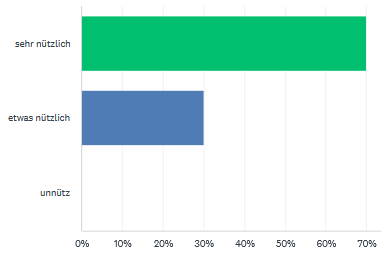
\includegraphics[width=0.40\textwidth]{images/frage-08}}
\end{wrapfigure}
\textbf{Ergebnisse:}\\
\\
\begin{tabular}{|l|c|}\hline
	\textbf{Antwortoptionen} & \textbf{Beantwortungen} \\\hline
	sehr nützlich  	& 7 \\\hline
	etwas nützlich	& 3 \\\hline
	unnütz 			& 0 \\\hline
	GESAMT			& 10 \\\hline			
\end{tabular}

\section{Frage 9}
\begin{wrapfigure}[2]{r}{0.5\textwidth}
	\centering
	\fbox{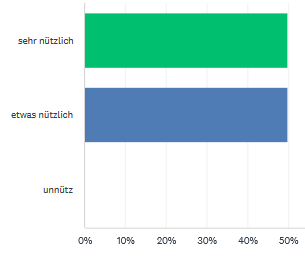
\includegraphics[width=0.40\textwidth]{images/frage-09}}
\end{wrapfigure}

\textbf{Frage:} Wie nützlich findest du DHBW Star?\\
\textbf{Ergebnisse:}\\
\\
\begin{tabular}{|l|c|}\hline
	\textbf{Antwortoptionen} & \textbf{Beantwortungen} \\\hline
	sehr nützlich  	& 5 \\\hline
	etwas nützlich	& 5 \\\hline
	unnütz 			& 0 \\\hline
	GESAMT			& 10 \\\hline			
\end{tabular}

\section{Frage 10}

\textbf{Frage:} Was Fehlt dir noch bei DHBW Star?\\
\textbf{Ergebnisse:}\\
\\
\begin{tabular}{|l|c|}\hline
	\textbf{Antwortoptionen} & \textbf{Beantwortungen} \\\hline
	Integration von Dualis  	& 7 \\\hline
	Integration von Moodle 	& 4 \\\hline
	Integration ÖPNV Fahrplan  			& 5 \\\hline
	Umfragen für Kurs Erstellen & 5 \\\hline
	Benachrichtigungen für Kurs  & 2 \\\hline
	Individueller Scheduler (Vorlesungen ein- und ausblenden,\\ eigene Termin hinzufügen) & 7 \\\hline
	Todo Liste (Hausaufgaben / Abgaben) & 2 \\\hline
	Sonstiges (bitte angeben)\\
	Wäre fürs 1.Semester sehr sinnvoll gewesen\\
	Wäre am anfang des studiums nützlich gewesen & 2 \\\hline 
	Befragte gesamt:			& 10 \\\hline			
\end{tabular}

\begin{figure}[htbp]
	\fbox{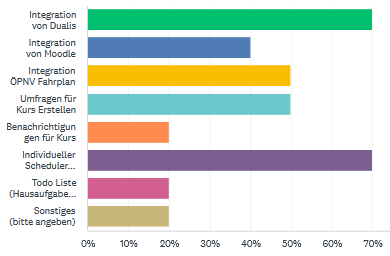
\includegraphics[width=\textwidth]{images/frage-10}}
\end{figure}